% Messwerte: Alle gemessenen Größen tabellarisch darstellen
% Auswertung: Berechnung geforderter Ergebnisse mit Schritten/Fehlerformeln/Erläuterung/Grafik (Programme)
\section{Auswertung}
\label{sec:auswertung}

\subsection{Fehlerrechnung}
\label{sec:Fehlerrechnung}
Die Fehlerrechnung, für die Bestimmung der Messunsicherheiten, wird mit Uncertainties \cite{uncertainties} gemacht.
Die Formel der Gauß Fehlerfortpflanzung ist gegeben durch
\begin{equation}
    \Delta f=\sqrt{\sum_{i=1}^N\left(\frac{\partial f}{\partial x_i}\right)^2 \cdot\left(\Delta x_i\right)^2}.
    \label{eqn:gauss}
\end{equation}
Für den Mittelwert gilt 
\begin{equation}
    \bar{x} = \frac{1}{N}\sum\limits_{i = 1}^N x_i .
    \label{eqn:mittelwert}
\end{equation}
Der Fehler des Mittelwertes ist gegeben durch 
\begin{equation}
    \Delta \bar{x}=\frac{1}{\sqrt{N}} \sqrt{\frac{1}{N-1} \sum_{i=1}^N\left(x_i-\bar{x}\right)^2}.
    \label{eqn:mittelwertfehler}
\end{equation}

\subsection{Vermessung des Acrylblocks mit einer Schieblehre}
\label{Vermessung des Acrylblocks mit einer Schieblehre}

\begin{figure}[H]
    \centering
    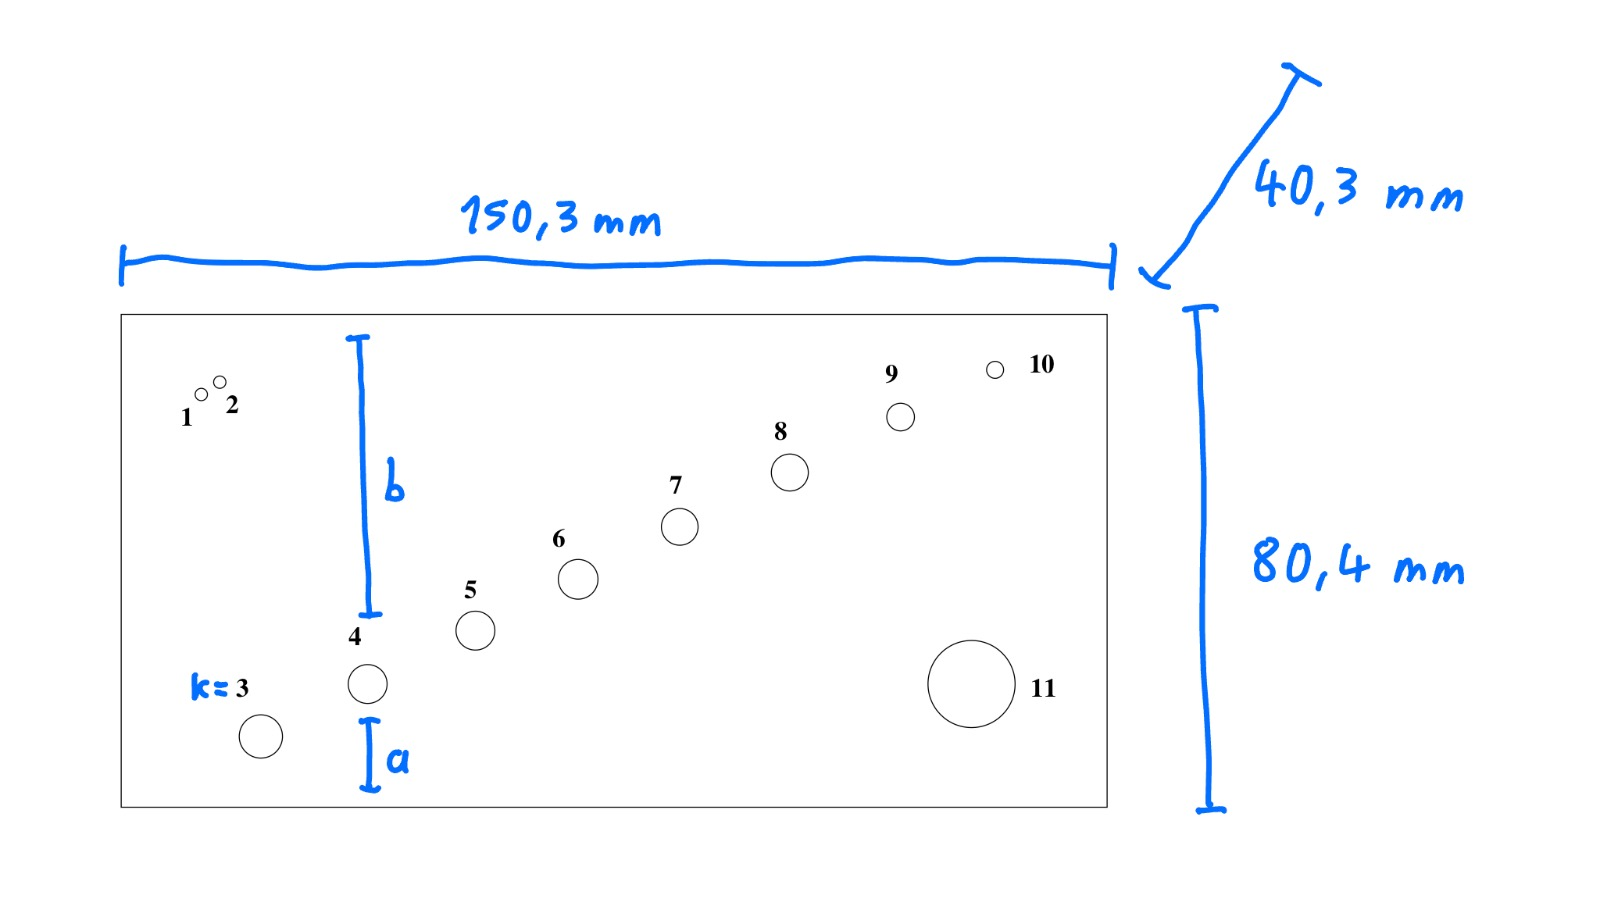
\includegraphics[width=0.9\linewidth]{content/grafik/abmessung.jpg}
	\captionsetup{width=0.765\linewidth}
    \label{fig:abmes}
\end{figure}

\begin{table}[H]
    \centering
    \caption{Abmessung der Löcher des Acrylblocks}
    \label{tab:lab}
\begin{tabular}{c c c c}
    \toprule
    Loch & $a_k$ & $b_k$ & d\\
    \midrule
    1 &     &       & 1.45 \\
    2 &     &       & 1.5 \\
    3 & 13.5 & 61.85 &    6  \\
    4 &21.85 &  54.4 &  4.9  \\
    5 &30.3 &  47.0 &    4  \\
    6 & 38.7 &  39.5 &  2.9  \\
    7 &46.8 &  31.0 &    3  \\
    8 &54.7 &  23.0 &  2.9  \\
    9 & 62.7 & 15.35 & 2.85  \\
    10 & 70.6 &   7.2 & 2.85  \\
    11 &15.2 &  55.8 &  9.5 \\
    \bottomrule
    \end{tabular}
\end{table}

\subsection{Untersuchung der Störstellen des Aceylblocks mit A-Scan}
\label{Untersuchung der Störstellen des Aceylblocks mit A-Scan}

\begin{tabular}{c c}
    \toprule
    Loch & $\text{Laufzeit} t / \si{\micro\second} $\\
    \midrule
     3 & 10.83 \\
     4 &  17.0 \\
     5 &  23.6 \\
     6 &  29.8 \\
     7 &  35.4 \\
     8 &  41.1 \\
     9 &  46.7 \\
    \bottomrule
\end{tabular}
